\begin{exercise}
      {ID-71ca299a0a3632bb0673afb32bb35f7ef7b12f58}
      {Zwei Münzen}
  \ifproblem\problem
    Zwei gleiche Münzen -- zum Beispiel zwei \eur{2} Münzen -- liegen wie es
    die Abbildung zeigt, auf dem Tisch. Die untere Münze wird festgehalten, und die
    obere wird am Umfang der anderen um sie herum gerollt, bis sie wieder oben an
    ihrer Ausgangsposition liegt. Wie oft hat sich dabei die obere Münze um sich
    selbst gedreht?
    \begin{center}
      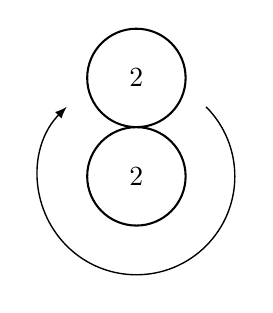
\begin{tikzpicture}[scale=1.25]
        \draw [line width=0.75pt] (0, 0) circle (0.5) node{\eur{2}};
        \draw [line width=0.75pt] (0, 1) circle (0.5) node{\eur{2}};
        \draw [line width=0.5pt, <-, >=latex, rotate=135] (1, 0) arc (0:270:1cm);
      \end{tikzpicture}
    \end{center}
  \fi
  \ifoutline\outline
    Stelle dir zunächst vor, dass die gerollte Münze auf dem Zeiger einer Uhr
    festgeklebt worden wäre\ldots
  \fi
  %\ifoutcome\outcome
  %\fi
\end{exercise}
